In this section, we present the model of the hybrid dynamical system
under test, and the background for PWA relational abstractions.


\subsection{System-under-test ($\System$)}

We assume that the system-under-test is a hybrid dynamical system, \ie, a
system which has discrete modes and a continuous state-space, and which
evolvution is either (1) continuous in time according to the dynamics
associated with its current discrete mode (typically described using
differential equations over its continuous state), or (2) through
discrete jumps that possibly change the discrete mode of the system and
possibly reset its continuous state to some value.  However, we assume
that the system is {\em effectively black-box}. This means that we do not
assume any knowledge of the symbolic dynamical equations describing the
system behavior. We do assume some knowledge of the system: an {\em
interface} view, in which we are allowed to stimulate the system with
inputs and observe its outputs. 

We formally define a system-under-test $\System$ as a tuple $(\Modes,
\ContStates, \initmode, \initstate, \Delta, \Inputs, \Outputs)$.  Here,
system state-space (denoted $\HybridStates$) is a subset of $\Modes \times
\ContStates$, where $\Modes$ is a finite set of discrete modes, and
$\ContStates$ is a compact subset of $\Reals^n$ representing the set of
continuous states.  We assume that the system is {\em initialized} to an
initial mode $\initmode$ and an initial state $\initstate$ at time $t=0$.
We assume that the system has $m$ exogenuous inputs which take values from
the set $\Inputs$ which is a compact subset of $\Reals^m$. We assume that
the system has $\ell \le n$ outputs, where $\Outputs \subseteq
\HybridStates$. In this paper, we assume that the entire system state is
observable.  In other words, $\Outputs = \HybridStates$. 

Finally, we restrict our attention to switched-mode systems, \ie, those in
which there is a partition imposed on $\ContStates$, and there is a
bijective map between each element $\ContStates_i$ in the partition and
each mode in $\Modes$.

The operational semantics of $\System$ is defined in terms of a
forward-simulation map $\simmap_\Delta$, which is a function that maps a
time $t$, the current state of the system, and an input value in $\Inputs$
to the state of the system at time $t+\Delta$.




% We assume that $\System$ is a hybrid dynamical system with exogenous
% inputs modeling an embedded control system. 
% 
% we assume that the hybrid system is effectively a switched-mode
% dynamical system, \ie, the mode of the system is completely determined
% by its state.  An input to $\System$ is assumed to be a time-bounded
% {\em signal}, \ie, a function from $[0,T]$ to $\Inputs$, with $T$ as
% the time horizon, and $\Inputs \subseteq \Reals^k$.  In this paper, we
% view $\System$ as effectively black-box equipped with a forward
% simulation map, in a simulation time-step of $\Delta_t$ from time $t$,
% allows computing the unique reachable state $\vx \in \HybridStates$
% given state-input pair $(\vx,\vu)$.

% time and input parameterized reachability relation $\reach{t,
% \vu}_\System \subseteq \HybridStates \times \HybridStates$ as follows:
% $\simulate^{\System}:
% (\vx, \vu, t) \mapsto \vx$, where $\vx \in \HybridStates$, $\vu \in
% \Inputs$ and $t \in [0,T]$.


% Given the hybrid state space $\vx\in\HybridStates$ and input space $u
% \in\Inputs$ and time step $t$, it computes the unique successor state
% $\vy=\simulate^{\System}(\vx,u,t)$ such that $\vx \reach{t,u} \vy$.


\begin{definition}[System Evolution]
    The behavior of system $\System$ at time $t$ is described as an
    evolution in the hybrid state-space $\HybridStates$ under the
    effect of the input $\vu \in \Inputs$ at time $t$. The forward
    simulation map $\mathsc{sim}^\System : \HybridStates \times \Inputs
    \times \Reals^+ \mapsto \HybridStates$, maps a state $\x\in\HybridStates$ at time
    $t$ to a new state $\x'\in\HybridStates$ at time $t+\Delta\in\Reals^+$, under a constant
    input $\vu$.  Finally, we define the time and input parameterized
    reachability relation $\reach{t,u} \subseteq \HybridStates \times
    \HybridStates$ such that
    \begin{equation}
        (\vx,\vx') \in \reach{t,u} \;\text{iff}\; \vx'=\mathsc{sim}^{\System}(\vx,u,t).
    \end{equation}
\end{definition}

\mypara{System Assumptions:} We require that $\System$ can always be
simulated forward in time with deterministic results. This in turn
requires existence and uniqueness of trajectories over a finite time
horizon $[0,T]$, which can be guaranteed by Lipschitz continuity of
the vector field in each underlying hybrid mode, ruling away issues
such as finite escape times~\cite{Meiss/2007/Differential}, and having
well-defined semantics for simulations at switching boundaries. While
these assumptions hold for the dynamical system examples which we
consider in this paper, such assumptions can be restrictive for
general control system models. When analyzing a system that does not
obey theoretical conditions that allow deterministic simulation, we
assume that the underlying tool used for numerical approximations of
system behaviors uses deterministic simulation semantics.  Finally, we
assume full observability of the system state, validate our results
only against the $\mathsc{sim}^\System$ function (as the analytic closed-form
representation of the system dynamics is assumed to be unavailable).
From here on, we drop the subscript $\System$ whenever it is clear
from the context. Also, to ease the presentation, we conflate the
inputs with the state and denote them by $\vx$.

\subsection{Graph Abstraction}

We base our methodology on the implicit discrete abstraction for
black-box dynamical systems~\cite{zutshi2014multiple}. The authors
showed how this abstraction is a graph abstraction, and reduced the
search for abstract violations to finding paths in a graph.

% Such an abstraction is defined by partitioning the
% state-space of the system using a grid, and hence each abstract state
% is a hyper-rectangle. The relations between abstract states are
% obtained by suitably lifting $(\vx,\vx') \in\reach{t,u}$. Considering
% the abstract states as vertices of a graph and the relations as edges
% between nodes, the problem of finding an abstract counter-example
% (CEx) can be cast as finding a path in the graph. Such an abstraction
% can be explored on-the-fly by enumerating the abstract relations
% between a pair of states.

\mypara{A discrete abstraction} over a continuous space uses relations
to describe the behavior of the system over time. Such relations
abstract the underlying relation between concrete states, and concrete
paths can no longer be constructed directly. Instead, search
procedures like Counter-Example Guided Refinement (CEGAR) must be used
to find concrete paths. In general, such search techniques are based
on refinement of the state-space and exponential with respect to
computational resources and memory. As an alternative, we introduce
data driven `enrichment' of abstractions to approximate the concrete
relations underlying the abstract relations.  Specifically, we use
linear regression to compute affine maps associated with the relations
between two abstract states. We then show how associating the computed
maps with the relations transforms a discrete abstraction into a PWA
transition system.

% The abstraction of the hybrid dynamical system is a a
% partitioning of the combined state-input space $\HybridStates \times
% \Inputs$ into hyper-rectangles or cells $C_i \in \Cells$. The cells are
% pairwise disjoint $C_i \cap C_j \neq \emptyset$ iff $i \neq j$ and
% their union $\bigcup_{C_i\in\Cells}C_i$ is the state-input
% space $\HybridStates \times \Inputs$. The partitions over
% the continuous input-state space are implicitly defined using a quantization
% function $Q_\epsilon$ parameterized by the precision $\epsilon$.
% This further defines an equivalence relations such that
% \[
%     (\vx_i, \vu_i) \equiv (\vx_j, \vu_j) \;\text{iff}\; Q_\epsilon(\vx_i,
%     \vu_i) = Q_\epsilon(\vx_j, \vu_j)
% \]
% In other words, $(\vx_i, \vu_i) \in C_i \; \text{iff} \; C_i =
% Q_\epsilon(\vx_i, \vu_i)$.

% \begin{definition}[Graph Abstraction]
%     The quantization function $Q_\epsilon$ induces a DAG on the discrete
%     abstraction given by a graph $G(V, E)$, where each vertex
%     corresponds to a cell $V_i = C$, and an edge exists between two
%     cells $(C, C') \in E_i$ iff there exist state-input pairs
%     $(\vx,\vu) \in C$, $(\vx', \vu) \in C'$ such that $\vx' =
%     \simulate(\vx, \vu )$.
% \end{definition}

The abstraction of the hybrid dynamical system is a a partitioning of
the hybrid state space $\HybridStates$ into hyper-rectangles or cells
$C_i \in \Cells$. The cells are pairwise disjoint $C_i \cap C_j \neq
\emptyset$ iff $i \neq j$ and their union $\bigcup_{C_i\in\Cells}C_i$
is the state space $\HybridStates$. The partitions over the continuous
state space are implicitly defined using a quantization function
$Q_\epsilon$ parameterized by the precision $\epsilon$.  This further
defines an equivalence relations such that $(\vx_i) \equiv (\vx_j)
\;\text{iff}\; Q_\epsilon(\vx_i) = Q_\epsilon(\vx_j)$.  In other
words, $(\vx_i) \in C_i \; \text{iff} \; C_i = Q_\epsilon(\vx_i)$. The
abstraction can be interpreted as a graph and explored using fixed
time $(\Delta\in\Reals^+)$ relations obtained using
$\simulate(\vx)$~\footnote{$\simulate(\vx)$ is a fixed
parameterization of $\mathsc{sim}(\vx,\Delta)$}.

\begin{definition}[Graph Abstraction]
    The quantization function $Q_\epsilon$ induces a directed acyclic
    graph (DAG) on the discrete
    abstraction given by a graph $G(V, E)$, where each vertex
    corresponds to a cell $V_i = C$, and an edge exists between two
    cells $(C, C') \in E_i$ iff there exist state-input pairs
    $(\vx) \in C$, $(\vx') \in C'$ such that $\vx' =
    \simulate(\vx)$.
\end{definition}



Given a numerical simulator $\simulate$ and an initial abstraction
defined by a quantization function $\quant_\epsilon$ and a time step
$\Delta$, we pick samples and simulate them to explore the abstraction
on the fly to obtain a graph $G$, which has a finite number of
abstract states $C$ (or cells) and edges $(C,C')$ iff $C
\areach{\Delta} C'$.


% \begin{definition}[Abstract State Graph]. Let ∆ > 0 be a fixed time
%     step. The abstract state graph H(∆) for time step ∆ is defined by
%     the set of vertices C, and edges (Ci, Cj ) whenever Ci ∆ Cj . Let
%     C0 denote the collection of initial cells in C, i.e., cells Ci
%     such that Ci ∩ X0 6= ∅. Further, let Cu denote the set of unsafe
%     cells, or cells Cj such that there is a state xj ∈ Cj that reaches
%     an unsafe state y ∈ Xf within time 0 ≤ tj < ∆. The abstraction
% H(∆) is given by D C, ∆ , C0, Cu E .  \end{definition}

Instead of using a CEGAR like loop (used in~\cite{zutshi2014multiple}),
we use the generated trajectories to learn quantitative models
describing the local behavior of the system. These models are defined
by a set of relations $R \subseteq \HybridStates \times \HybridStates$
for each edge of the reachability graph. In the next section, we
summarize this idea.


\subsection{Enriched Abstraction}


\begin{figure}[!htbp]
\begin{center}
\tikzstyle{line} = [thick]
\tikzstyle{arw} = [->, thick,>=stealth,shorten <=2pt, shorten >=2pt]
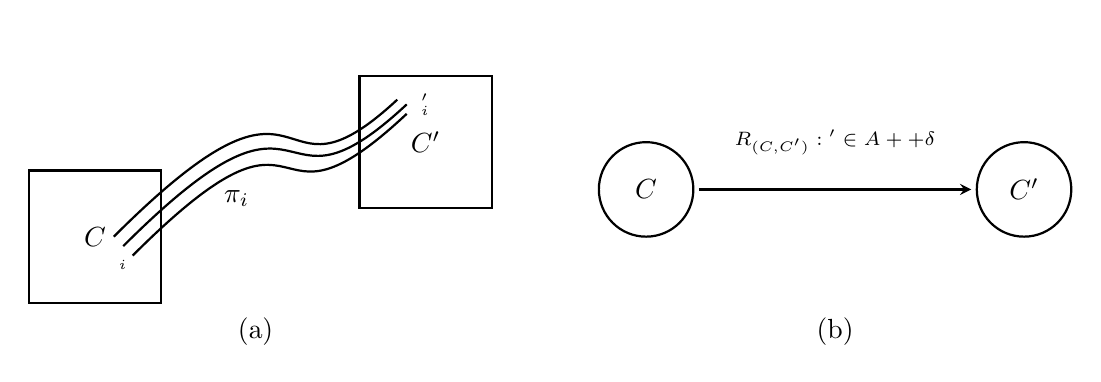
\begin{tikzpicture}
\begin{scope}[scale=1.2]

    \draw [line] (-5.2,-1.2) rectangle (-3.8,0.2);
    \draw [line] (-1.7,-0.2) rectangle (-0.3,1.2);
    \draw [line] (-4.1,-0.7) .. controls +(2.0,2.0) and +(-1.6,-1.5) ..  (-1.2,0.8);
    \draw [line] (-4.2,-0.6) .. controls +(2.1,2.1) and +(-1.5,-1.4) ..  (-1.2,0.9);
    \draw [line] (-4.3,-0.5) .. controls +(2.2,2.2) and +(-1.4,-1.3) ..  (-1.3,0.95);

\node at (-4.5, -0.5) {$C$};
\node at (-1, 0.5) {$C'$};
\node at (-4.2,-0.8) {\scriptsize{$\x_i$}};
\node at (-1.0,0.90) {\scriptsize{$\x_i'$}};
\node at (-3,-0.1) {$\pi_i$};
\node at (-2.8, -1.5) {(a)};
\end{scope}

\begin{scope}[xshift=4.0cm,scale=1.2]
\draw [line] (-2.0,0) circle (0.5);
\draw [line] (2.0,0) circle (0.5);
\draw[arw] (-1.5,0) -- (1.5,0);
\node at (-2.0,0) {$C$};
\node at (2.0,0) {$C'$};
\node at (0,0.5) {\scriptsize{$R_{(C,C')}:\setof{\x' \in A\x + \vb + \delta}$}};
\node at (0.,-1.5) {(b)};
\end{scope}
\end{tikzpicture}
\end{center}
\vspace*{-.3cm}
\caption{(a) Trajectory segments $\traj_i$ are used to compute the
relation $R_{(C,C')}$ that annotates the edge in (b).
$R_{(C,C')}:\setof{\x' \in A\x + \vb + \delta}$ is an interval affine
relation defined by an affine map (matrix $A$ and vector $\vb$) and an
error interval (vector of intervals $\delta$).}
    \label{fig:enriched-edge}
\vspace*{-.3cm}
 \end{figure}


Recall that each edge $(C,C')$ of the graph $G$ denotes an observed
trajectory between the respective cells. The graph abstraction $G$
only states that there exists a state $\x \in C$ from which the system
can evolve to a future state $\x' \in C'$. To increase the precision,
iterative refinement of the abstraction by state splitting was
proposed in~\cite{zutshi2014multiple}. Due to the curse of
dimensionality, state splitting is not scalable. Instead, we propose
an `enrichment' $G^R$ of $G$ by computing a set of local relations
$R_{(C,C')}(\x,\x')$ for every edge $(C,C')$, which
non-deterministically describe relations between $\x \in C$ and $\x'
\in C'$. This is illustrated in \figref{enriched-edge}.
%(compare with \figref{segtraj}).

The enriched graph $G^R$ captures the underlying local forward
dynamics describing the evolution of the system in each abstract
state. We represent the dynamics using an affine model with an
interval error. Such a model can either be approximated using learning
methods or computed as a sound (over) approximation using reachability
set computation methods. Because we assume black box semantics, we
only present the former. Using regression analysis on a witnessed
trajectory between two cells, we compute an approximate discrete map
along with an error estimate.  Moreover, using the simulation function
$\simulate$, additional trajectories (or data) can be generated if
required. The data can be separated into a training set and testing
set to compute the map and the error respectively.

%The latter case can be explored if
%the symbolic dynamics of the system are known. A tool like
%\flowstar~\cite{chen2013flow} can be used to find the reachable set
%map.

Observe that $G^R$, a directed reachability graph, is rich enough to
search for concrete behaviors in the system. We call it a time
parameterized PWA relational abstraction. It can be interpreted as an
infinite state discrete transition system, and we can use
off-the-shelf bounded model checkers to find concrete violations of a
given safety property, and even other temporal properties.

\begin{figure}[!htbp]
\begin{center}
\tikzstyle{line} = [thick]
\tikzstyle{arw} = [->, thick,>=stealth,shorten <=2pt, shorten >=2pt]
\tikzstyle{block} = [rectangle, minimum width=0.5cm, minimum height=1.0cm, text centered, draw=black, align=center]%, fill=blue!25]
\begin{tikzpicture}[scale=1.0, on grid, auto]

    \node (G) at (-4,0) {$G$};
    \node (GR) at (0,0) {$G^R$};
    \node (CEX) at (4,0) {$CEx$};

    \node (enrich) [block] at (-2, 0) {\scriptsize Enrich using \\ \scriptsize affine  maps};
    \node (BMC) [block] at (2, 0) {\scriptsize Find CEx \\ \scriptsize using BMC};

    %\node[align=center] at (0, 0) {\scriptsize Enrich using \\ \scriptsize Regression \\ \scriptsize(OLS)};

    %\draw [line] (-2.0,-0.5) rectangle (-1.0,0.5);
    \draw[arw] (G.east) -- (enrich.west);
    \draw[arw] (enrich.east) -- (GR.west);
    \draw[arw] (GR.east) -- (BMC.west);
    \draw[arw] (BMC.east) -- (CEX.west);

\end{tikzpicture}
\end{center}
\vspace*{-.3cm}
\caption{Finding counter-examples (CEx) in a graph abstraction using PWA models.}
\label{fig:overview}
\vspace*{-.3cm}
\end{figure}
